\chapter{Propuesta o tema central de la tesis}
\pagenumbering{arabic}
\setcounter{page}{16}
\renewcommand{\baselinestretch}{2} %doble espacio paratodo el texto

{\bf Ejemplo:}\par

Basado en los conceptos discutidos en los capítulos 1 y 2, así como de la experiencia obtenida del análisis de resultados de los modelos matemáticos estudiados y programados con CPLEX, se caracterizan los principales elementos que componen el modelo propuesto en este trabajo para la colecta y transporte de RSU en un área urbana. Así, se estructura una red logística reversa para los RSU considerando diferentes centros especializados o unidades  productivas para atender las diferentes fases del proceso en la red. En este proceso de modelamiento se tuvo cuidado en mantener la propuesta lo mas cerca a la realidad de las ciudades, donde el modelo fue testado y validado.

\section{Proceso de modelamiento} 

{\bf Ejemplo:}\par

La planificación y modelamiento del sistema de logística reversa de una área urbana es una fase importante y estratégica, para obtener en el futuro óptimos resultados en el proceso de gerenciamiento y operación del sistema reverso de RSU. El modelamiento permite determinar la localización de las estaciones de colecta y de unidades especiales necesarias, asi como el flujo que será movido a los largo de la red permitiendo dimensionar todo el sistema y sus componentes (Figura 3.1).
\vskip 0.3cm
\begin{figure}[ht]
\begin{center}
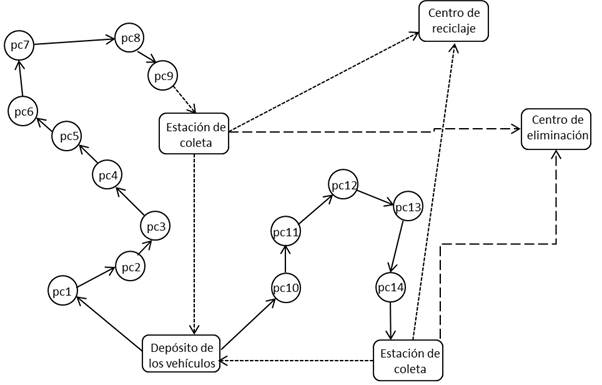
\includegraphics[width=.6\textwidth]{Figura3}
\end{center}
\begin{center}
\vskip -0.5cm
\caption{\small{Esquema del proceso de colecta y transporte de RSU.}}
{\small{Fuente: Elaboración propia}}
\end{center}
\end{figure}

\subsection{Proceso de ruteo}

